\lstdefinelanguage{plaintext}{
  sensitive=false,
  comment=[l]{//},
  morecomment=[s]{/*}{*/},
  identifierstyle=\color{black},
  morestring=[b]',
  morestring=[b]"
}

\lstset
{ 
    language=plaintext,
    basicstyle=\footnotesize,
    numbers=left,
    stepnumber=1,
    showstringspaces=false,
    tabsize=1,
    breaklines=true,
    breakatwhitespace=false,
    frame=leftline
}

\chapter{Implementasi dan Pengujian}
\label{chap:implementasiDanPengujian}

Pada bab ini dibahas mengenai implementasi perangkat lunak dan pengujian yang dilakukan terhadap perangkat lunak tersebut. Lingkungan implementasi, yang meliputi perangkat keras dan perangkat lunak, serta hasil implementasi akan dijelaskan pada bab ini. Selain Pengujian yang dilakukan pada skripsi ini, yang meliputi pengujian fungsional dan eksperimental akan dijelaskan pada bab ini.

\section{Implementasi}
Pada bagian ini akan dijelaskan mengenai lingkungan yang digunakan untuk membangun perangkat lunak beserta hasil implementasinya.

\subsection{Lingkungan Implementasi}
Berikut spesifikasi perangkat keras dan perangkat lunak yang digunakan dalam pembangunan pada skripsi ini:

\begin{enumerate}
	\item Spesifikasi Perangkat Keras
	
		\begin{itemize}
			\item Perangkat: Laptop
			\item Processor: AMD Bristol Ridge Quad Core FX-9830P 3GHz
			\item RAM: 8GB
			\item GPU: Radeon RX 460
			\item Storage: Harddisk 1TB
		\end{itemize}		

	\item Spesifikasi Perangkat Lunak

		\begin{itemize}
			\item Sistem Operasi Windows 10 64-bit
			\item PHP 7.3.5 (cli)
			\item Composer versi 1.8.5
			\item Sublime Text versi 3.2.1
		\end{itemize}	
	
\end{enumerate}

\subsection{Hasil Implementasi}
Perangkat lunak dikembangkan menggunakan bahasa pemrograman PHP. Perangkat lunak yang dibuat tidak menggunakan \textit{Graphical User Interface}, melainkan berbasis \textit{Command Line Interface}. Perangkat lunak akan menerima input berupa file PDF skripsi yang disimpan pada folder yang telah disediakan, dan mengeluarkan laporan kesalahan pada terminal.

\begin{figure}[H]
	\centering	
	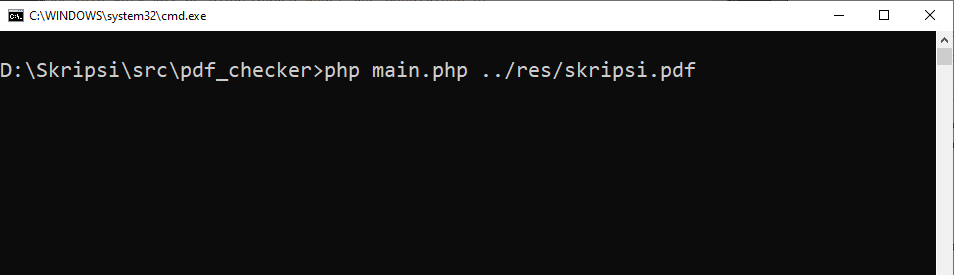
\includegraphics[scale=0.6]{command.png}
	\caption{Perintah yang digunakan untuk menjalankan perangkat lunak}	
	\label{fig:command} 
\end{figure}

Gambar \ref{fig:command} merupakan perintah yang perlu dituliskan pada terminal, untuk menjalankan perangkat lunak. Kelas Main menjadi kelas yang digunakan untuk menjalankan seluruh proses yang berjalan dalam perangkat lunak. File PDF skripsi yang akan diperiksa harus berada di folder yang telah disediakan, yaitu pada folder Skripsi$\backslash$src$\backslash$res.

\section{Pengujian}
Pada bagian ini akan dijelaskan mengenai pengujian yang dilakukan pada perangkat lunak. Akan dilakukan 2 bentuk pengujian pada skripsi ini, yaitu pengujian fungsional dan pengujian eksperimental.

\subsection{Pengujian Fungsional}
Pengujian fungsional bertujuan untuk menguji fungsionalitas perangkat lunak. Perangkat lunak memiliki 8 fitur yang telah diimplementasikan. Fitur-fitur tersebut akan diuji untuk melihat kebenaran dan kesesuaian fitur tersebut dengan yang diharapkan.

\subsection{Pengujian Eksperimental}
